\documentclass{beamer}

% \usepackage{beamerthemesplit} // Activate for custom appearance

\usetheme{Szeged}
\usefonttheme{professionalfonts}
\usecolortheme{rose}

\title{Creating and Updating}
\author{James Condron}
\date{\today}

\begin{document}

\frame{\titlepage}

\section{Intro}
\frame{
  \frametitle{Basics and CRUD}
  {\Large C} reate    \\
  {\Large R} ead      \\
  {\Large U} pdate   \\
  {\Large D} elete
}

\frame{ 
  \tableofcontents
}

\subsection{Overview}
\frame{
  \frametitle{Touching the shiny data}
  \begin{itemize}
    \item <1-> Creating records
    \item <2-> Updating records
    \item <3-> Constraints
  \end{itemize}
}

\section{Practicals}
\subsection{Creating}
\frame{
  \frametitle{Create}
  We use the {\tt insert} verb \\
  We can insert in one of two ways;
  \begin{itemize}
    \item <1-> {\tt insert}ing by specifying the columns we're
      inserting into
    \item <2-> {\tt insert}ing into every column in the right order
  \end{itemize}
}
\frame{
  \frametitle{Create (cont.)}
  \begin{itemize}
    \item <1-> {\tt insert into my\_table values (100, 'Eli', '56 Tudor Court',
      'Feta');}
    \item <2-> {\tt insert into my\_table (name, favourite\_cheese,
        address) values ('Eli', 'Feta', '56 Tudor Court');}
  \end{itemize}
}

\subsection{Updating}
\frame{
  \frametitle{Update}
  We use the verbs {\tt update} and {\tt set} together with a {\tt
    where} \\
  In one line we tell the database what we want to search for and what
  we want to replace
}
\frame{
  \frametitle{Update (cont.)}
  \begin{itemize}
    \item <1-> {\tt update my\_table set a\_column='poop' where
        a\_column = 'poo poo'}
    \item <2-> {\tt update my\_table set a\_column='poop' where
        a\_column like 'poo\%'}
  \end{itemize}
}

\subsection{Constraints}
\frame{
  \frametitle{constraints}
  Constraints limit (`constrain') what records can fit a column \\
  These affect our inserts and updates
}
\frame{
  \frametitle{constraints (cont.)}
    \begin{figure}[h]
     \centering
     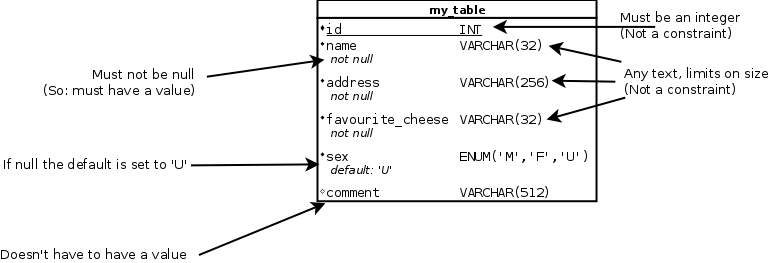
\includegraphics[width=4.5in]{images/constraints.png}
     \caption{Constraints on my\_table}
     \label{fig:constraints}
  \end{figure}
}

\end{document}
